\section{Epigenetic Data}
In order to train and compare our single-tasks and multi-tasks neural networks explained in Chapter~\ref{cap:methods} we built a dataset of epigenetic data. We gathered the epigenetic features data from
ENCODE \cite{ENCODE_data} and the enhancers and promoters labels from
FANTOM \cite{FANTOM_data}. Formally we can define our data as follow: 
\begin{itemize}
    \item $L$ is the set of \emph{cell lines};
    \item $C$ is the set of \emph{chromosomes};
    \item $I$ is the set of \emph{intervals} over the natural numbers;
    \item $S_\ell\subseteq C\times I$, $\ell\in L$, is the set of \emph{sequences} (pair of chromosomes and intervals) relative to the cell line $\ell$, which can be mapped injectively to sequences of 1000; in general, $S_\ell\neq S_{\ell'}$; the mapping to the nucleotides is dependent on the pair chromosome/interval only;
    \item $Y$ is the set of \emph{labels} from FANTOM that can be associated to sequences (e.g., active promoter);
    \item for each $\ell\in L$, $F_\ell$ is a set of \emph{features} and $e_\ell:S_\ell\to\mathbb R^{F_\ell}$ is a map representing ENCODE \emph{epigenetic data};
\end{itemize}
%TODO: check cell lines description correctness 
The set of cell lines $L$ includes: \emph{A549} a lung carcinoma cell line derived from old Caucasian male, \emph{GM12878} a lymphoblastoid cell line produced from the blood of a female donor with northern and western European ancestry by EBV transformation, \emph{H1} an human embryonic stem cell line, \emph{HEK293} a human embryonic kidney cell line, \emph{HEPG2} a cell line derived from a male patient with liver carcinoma, \emph{K562} an immortalized cell line produced from a female patient with chronic myelogenous leukemia and \emph{MCF7} a mammary gland adenocarcinoma cell line. For every cell lines $\ell \in L$, the set of sequences $S_\ell$ contains the genomics locations of enhancers and promoters. $Y$ contains the four classes of labeled regions, including \emph{active enhancers} (A-E), \emph{active promoters} (A-P), \emph{inactive enhancers} (I-E), \emph{inactive promoters} (I-P). A-E and I-E labels are defined as FANTOM enhancers with $TPM>0$ (tags per million) and $TPM=0$, respectively. A-P and I-P labels, instead, are promoters with $TPM>5$ and $TPM=0$. 
% Todo: Ultima frase presa da spiegazione di paper wasserman, cos'è TPM?! lo spiego?

%TODO: sistemare con riferimenti per uso media e mediana per l'imputer
For every cell line $\ell \in L$, the number of features $| F_\ell |$ are reported in Table~\ref{tab:featuressize}. It can be noted that, some cell lines, such as K562, HepG2 and HEK293 contains more than 200 features, in Section~\ref{sec:featureselection} we reported the approach followed in order to select a subset of discriminative features.
Note that, for every cell lines $\ell \in L$, in vitro experiments are
performed for every nucleotides of sequences. Consequently the pure ENCODE
data, for every sequence $s \in S_\ell$ and epigenomic feature $f \in
F_\ell$ (e.g., POLR2A), are represented by a $|s|$-length vectors of real
numbers. Those values must be summarized in a single metrics. The most
common used metrics are mean, variance and maximum, we choose to use
maximum. Moreover we have a very small percentage (less than 1\%) of
missing values; thus, we used as substitute the median of the others
values.
\begin{table}[t]
\centering
\begin{tabular}{|l|l|l|}
\hline
\textbf{Cell lines ($\ell \in L$)} & \textbf{$|F_\ell|$} & \textbf{$|F_\ell^{i^{*}}|$} \\ \hline
A549               & 54 & 14                  \\ \hline
GM12878            & 110 & 38                 \\ \hline
H1                 & 43 & 20                  \\ \hline
HEK293             & 207 & 35                 \\ \hline
HepG2              & 209 & 21                 \\ \hline
K562               & 320 & 36                 \\ \hline
MCF7               & 101 & 19                 \\ \hline
\end{tabular}
\caption{Original feature set and number of features selected for every cell line in $L$ compared}
\label{tab:featuressize}
\end{table}
\subsection{Computational Tasks}
To evaluate the performance of out models to discriminate between the different cis-regulatory regions labels $Y$ we proposed a group of \emph{computational problems}. Formally, given the set of labels $Y$, they are defined as a set of binary tuples $P \subseteq Y \times Y$; In particular $P$ contains the following tuples: 
\begin{itemize}
    \item Active Enhancers vs Active Promoters (A-E vs A-P);
    \item Active Promoters vs Inactive Promoters (A-P vs I-P);
    \item Active Enhancers vs Inactive Enhancers (A-E vs I-E); 
    \item Inactive Enhancers vs Inactive Promoters (I-E vs I-P); 
    \item Active Enhancers and Active Promoters vs Background (A-E+A-P vs BG).
\end{itemize}
In terms of classification, we considered the first and the second element of every items as the positive and negative training classes; thus, for instance, A-E and A-P are considered as positive and negative example, respectively. The last item is built by joining in positive class A-E and A-P labels and in negative class all the other labels. In other terms BG is composed by I-E and I-P labels. The performance of every computational problems are evaluated for every cell line $\ell \in L$. Thus we define a \emph{tasks} as a pair $p \in P \times L$. 

\section{Feature Selection} \label{sec:featureselection}
As previously described, in the problem at the hand we have a different set of epigenomic features $F_\ell$ for every cell line $\ell \in L$. As shown in Table~\ref{tab:featuressize}, some cell lines have a considerable size set of features, so many features might arise to a performance degradation of the models due to, for instance, to over-fitting. During the years many methods were developed to deal with large dimensional features sets, in this Section is given a detailed explanation of the feature selection approach followed in this work and the results it produced. 

Firstly, we tried to understand, for every cell lines, the number of features to select. To do this we use a well-known algorithm called Recursive Feature Elimination (RFE) \cite{VapnikRFE}. Given a model that assign weights to the features, RFE use them to recursively remove the least important feature until the last one. In this way, for every iterations $i$, we obtain a subset of features $F_{\ell}^{i} \subset F_\ell$. Note that the obtained subset are nested, $F_{\ell}^{1}  \subset  F_{\ell}^{2} \subset \cdots \subset F_{\ell}$. In order to obtain more accurate results, every RFE run is cross-validated. For every tasks $p \in P \times L$ and for every feature subset $F_\ell^i$ we computed the function of \emph{f1-score} values against the number of best features. With the increasing of the best features selected the best number of features the performance of the model should increase until a certain limit (the maximum of the function) and reach a plateau or in some cases decrease. Thus, given $i^{*}$ the index of the best subset iteration, the optimal number of feature $|F_\ell^{i^{*}}|$ for a certain task could be selected looking at the maximum of this function. In Figure~\ref{fig:feats_plot} are reported the obtained results, every plot consider a cell lines and every curve is a particular task $p$, the colored and black dotted vertical lines indicate respectively the maximum \emph{f1-score} for a given task and the mean. 

After fixing the number of features that should be considered for every cell lines (Table~\ref{tab:featuressize}) we tried to understand which features must be selected. Many methods could be found in literature in order to choose an optimal subset of features of given size, they are mainly divided into: \emph{filters} methods that rank features computing correlation coefficients and \emph{wrapper} methods that use models to score subsets of features \cite{Guyon}. Every approach has its own advantages, in order to have a proper feature selection we choose to join many approach together, in particular: 
\begin{itemize}
    \item \textit{Correlations with target}: it is a filter based method, Pearson correlation is computed for every features $f \in F_\ell$ against the target labels. The correlations values are used to ranking the features;
    \item \textit{Random Forest Wrapper}: the features are ranked using the \emph{Gini importance} \cite{giniimportance} of the features calculated during the training of a Random Forest \cite{breiman2001random}; 
    \item \textit{Logistic Regression Wrapper}: similar to the Random Forest Wrapper but the features are ranked using the coefficient of the features in the decision function of a trained Linear Regressor.
    \item \emph{Recursive Feature Elimination}: in addition to using RFE for selecting the optimal number of features, we also used it to select an optimal subset of given dimension. 
\end{itemize}
For every cell lines $\ell \in L$ and every task $p \in P$ we build a binary matrix $I_\ell(|F_\ell|, 4)$, where we have the features on the rows and the four selection methods on the columns. For every rows $f$ and every columns $m$ the element $i_{fm}$ of $I$ is defined as follow: 
\[
    i_{fm} = \begin{cases} 1 & \mbox{if } f \mbox{ is selected by method } m \\ 0 & \mbox{otherwise} \end{cases}
\]

Counting the ones in every rows $f$ we have a measure, ranging from 0 to 4, of the importance of each feature. The obtained values are averaged for every tasks $p \in P \times L$. 
% TODO: put results in appendix?!

\begin{figure}[!htb]
    \centering
    \begin{subfigure}[b]{0.48\textwidth}
        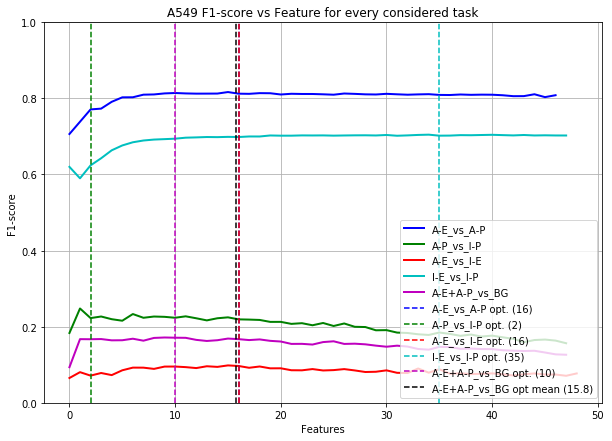
\includegraphics[width=\textwidth]{images/features_plots/A549_feature_plot.png}
        \caption{A549}
        \label{fig:A549_n_feat}
    \end{subfigure}
    ~ 
    \begin{subfigure}[b]{0.48\textwidth}
        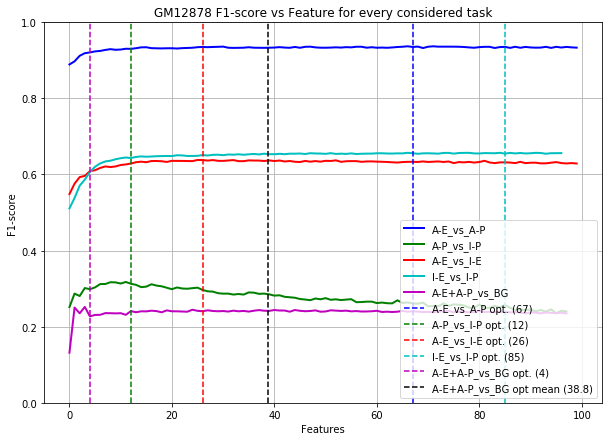
\includegraphics[width=\textwidth]{images/features_plots/GM12878_feature_plot.png}
        \caption{GM12878}
        \label{fig:GM12878_n_feat}
    \end{subfigure}
    ~ 
    \begin{subfigure}[b]{0.48\textwidth}
        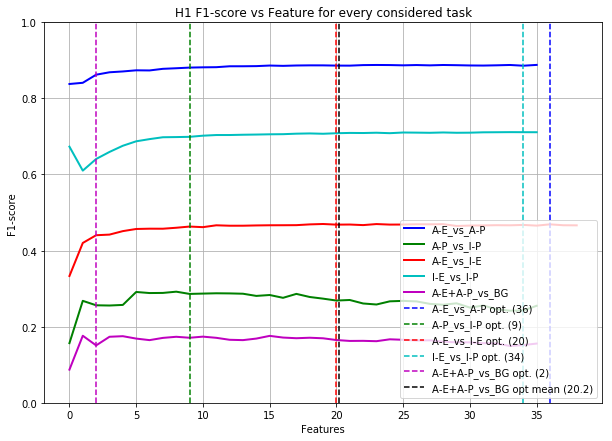
\includegraphics[width=\textwidth]{images/features_plots/H1_feature_plot.png}
        \caption{A mouse}
        \label{fig:H1_n_feat}
    \end{subfigure}
    \begin{subfigure}[b]{0.48\textwidth}
        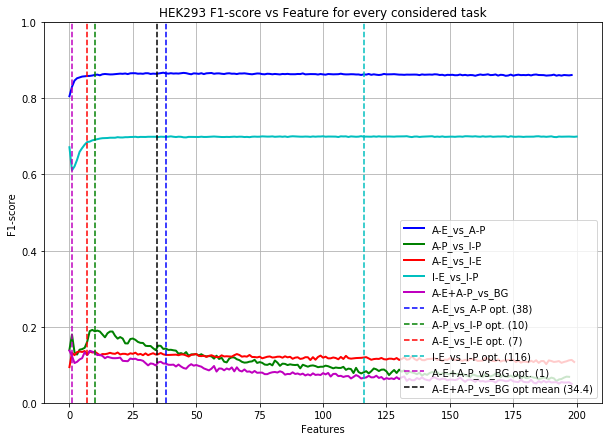
\includegraphics[width=\textwidth]{images/features_plots/HEK293_feature_plot.png}
        \caption{HEK293}
        \label{fig:HEK293_n_feat}
    \end{subfigure}
    
    \begin{subfigure}[b]{0.45\textwidth}
        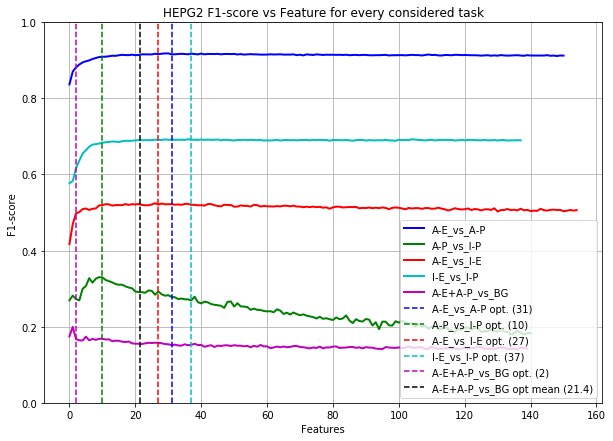
\includegraphics[width=\textwidth]{images/features_plots/HEPG2_feature_plot.png}
        \caption{HEPG2}
        \label{fig:HEPG2_n_feat}
    \end{subfigure}
    \begin{subfigure}[b]{0.48\textwidth}
        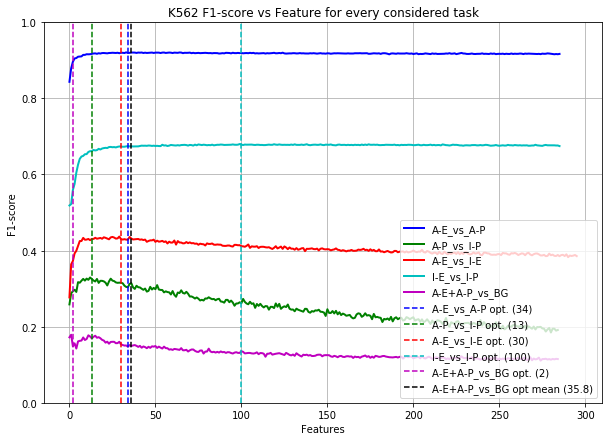
\includegraphics[width=\textwidth]{images/features_plots/K562_feature_plot.png}
        \caption{K562}
        \label{fig:K562_n_feat}
    \end{subfigure}
    
    \begin{subfigure}[b]{0.48\textwidth}
        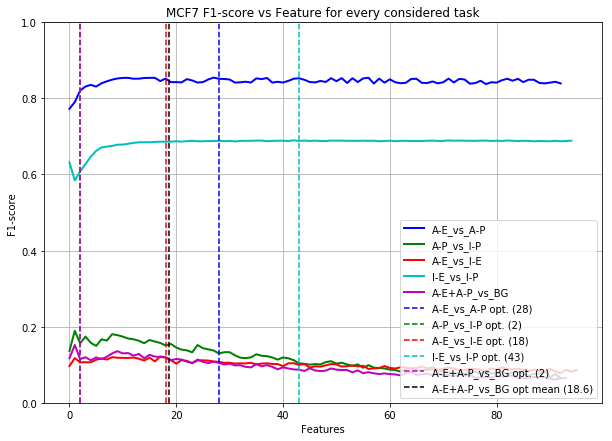
\includegraphics[width=\textwidth]{images/features_plots/MCF7_feature_plot.png}
        \caption{MCF7}
        \label{fig:MCF7_n_feat}
    \end{subfigure}
    \caption{Accuracy vs Number of Features plots for every $\ell in L$}\label{fig:feats_plot}
\end{figure}


\section{t-SNE Decomposition}
In order to have a general idea of the points separability we tried to  project them in a 2-dimensional space. Among many dimensionality reduction algorithm t-SNE were chosen. t-Distributed Stochastic Neighbor Embedding (t-SNE) \cite{vanDerMaaten2008} is an improvement of standard SNE \cite{HintonSNE} that allow a better cost function optimization. So, for every given task $p$, we  computed the t-SNE of every cell lines. 
In Appendix~\ref{appendix:tsne} are reported the results of analysis, every figure is a computational problem and every plot is a cell line $\ell$. We can notice that with the exception of A-E vs A-P (Figure~\ref{fig:tsneAEvsAP}) and A-E+A-P vs BG (Figure~\ref{fig:tsneAE+APvsBG}), respectively the least and the most numerous computational problems, all the other plots highlight the presence of evident clusters between positive (in blue) and negative (in red) labels. 